\documentclass[border=10pt]{standalone}
\usepackage{ifthen}
\usepackage{tikz}
\usetikzlibrary[
    decorations,
    decorations.pathmorphing,
    snakes,
]

\begin{document}

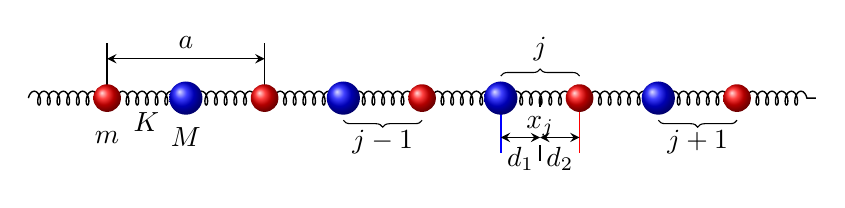
\begin{tikzpicture}
  [
  spring/.style={
    line width=0.5pt,
    decorate,
    decoration={
        coil,
        amplitude=2.5,
        segment length=3.5,
      }
    },
  ]
  \draw[line width=0.5pt] (1.0, 0.0) -- (1.0, 0.7);
  \draw[line width=0.5pt] (3.0, 0.0) -- (3.0, 0.7);
  \draw[line width=0.5pt, <->, >=stealth] (1.0, 0.5) -- node[pos=0.5, anchor=south] {$a$} (3.0, 0.5);

  \draw[line width=0.5pt, draw=black] (6.5, 0.0) -- (6.5,-0.8);
  \draw[line width=0.5pt, draw=blue] (6.0, 0.0) -- (6.0,-0.7);
  \draw[line width=0.5pt, draw=red] (7.0, 0.0) -- (7.0,-0.7);

  \node[below=3pt, fill=white] at (6.5, 0.0) {$x_j$};
  \draw[line width=0.5pt, <->, >=stealth] (6.0,-0.5) -- node[pos=0.5, anchor=north] {$d_1$} (6.5,-0.5);
  \draw[line width=0.5pt, <->, >=stealth] (6.5,-0.5) -- node[pos=0.5, anchor=north] {$d_2$} (7.0,-0.5);

  \node[anchor=center] at (1, -0.5) {$m$};
  \node[anchor=center] at (2, -0.5) {$M$};
  \node[] at (1.5,  -0.3) {$K$};

  \draw[decorate, decoration={brace, mirror, raise=8pt}] (4.0, 0.0) --
  node[pos=0.5, below=8pt] {$j-1$}(5.0, 0.0);
  \draw[decorate, decoration={brace, raise=8pt}] (6.0, 0.0) --
  node[pos=0.5, above=10pt] {$j$}(7.0, 0.0);
  \draw[decorate, decoration={brace, mirror, raise=8pt}] (8.0, 0.0) -- 
  node[pos=0.5, below=8pt] {$j+1$}(9.0, 0.0);

  \foreach \x in {0,1,...,9}{
    % draw the spring
    \draw[spring, draw=black] (\x, 0) -- ++(1, 0);
    % draw the atoms
    \ifthenelse{\x > 0}
    {
      \ifthenelse{\NOT \isodd{\x}}{
        \shade[ball color=blue] (\x, 0) circle (6pt);
      }{
        \shade[ball color=red] (\x, 0) circle (5pt);
      }
    }{}
  }
\end{tikzpicture}

\end{document}
